% ============================================================================
\section{Proposed System}
\label{sec:system}
% ============================================================================
The system separates two paths that meet in the knowledge base (Fig.~\ref{fig:architecture}). A language model takes part only in the knowledge-update path, which runs when a regulation or company policy is issued. The computation path runs at every payroll calculation and is deterministic.

\begin{figure*}[!t]
\centering
\figArchitecture
\caption{System architecture. The language model only drafts knowledge updates on the upper path; a reviewer approves them into the two-layer knowledge graph, and every computation on the lower path is deterministic and traced to legal provisions. Orange marks the language model, blue deterministic code, and green the human decision.}
\label{fig:architecture}
\end{figure*}

\subsection{Knowledge Representation}
\label{sec:representation}
GraphDB stores the structural knowledge as an RDF and OWL knowledge graph with SHACL validation and SPARQL queries (Fig.~\ref{fig:ontology}). The graph holds documents, provisions, quotes, rules, parameters, tables, company policies, change events, updates, and knowledge-base versions. The ontology reuses ELI for legal documents and provisions~\cite{publicationsoffice2026elien}, OWL-Time for validity intervals~\cite{cox2017owltime}, and PROV-O for the update that generated each element~\cite{lebo2013provo}. Each approved update becomes one named graph, so an earlier version of the knowledge base is a query over fewer graphs rather than a restored backup. The impact report and the trace query the graph for the rules that read a fact, the provision a value comes from, and the company rules that a change touches.

\begin{figure*}[!t]
\centering
\newcommand{\ontologicatatan}{Every pph:KBElement carries elementId, seq, recordedOn ($\approx$ prov:generatedAtTime), validFrom, and validUntil ($\approx$ time:ProperInterval);\\
   one named graph kb:update/\textit{id} per update. pph:Rule carries layer $\in$ \{Regulation, Company\}, modality $\in$ \{Mandatory, Default, Optional\},\\
   scope $\in$ \{Period, Year\}, expression, condition, fixed point, and policy.}
% Ontologi knowledge graph (docs/gambar/ontologi.tex) dengan label 8 pt Times sesuai templat IEEE.
% Keterangan di bawah gambar dapat diganti lewat \ontologicatatan (paper_en.tex memakainya).
\providecommand{\ontologicatatan}{Setiap pph:KBElement: elementId, seq, recordedOn ($\approx$ prov:generatedAtTime), validFrom, validUntil\\
   ($\approx$ time:ProperInterval); satu \en{named graph} kb:update/\textit{id} per pembaruan. pph:Rule: layer $\in$ \{Regulation, Company\},\\
   modality $\in$ \{Mandatory, Default, Optional\}, scope $\in$ \{Period, Year\}, expression, condition, fixed point, policy.}
\begin{tikzpicture}[
  node distance=6mm and 7mm,
  cls/.style={draw,rounded corners=2pt,fill=gray!8,font=\footnotesize,minimum height=5.5mm,inner sep=2.5pt},
  ext/.style={cls,fill=gray!20,dashed},
  sub/.style={-{Triangle[open]},thin},
  rel/.style={-{Stealth},thin},
  lab/.style={font=\footnotesize,fill=white,inner sep=0.8pt}]

% unsur knowledge base
\node[cls] (el) {pph:KBElement};
\node[cls,below left=9mm and 22mm of el] (rule) {pph:Rule};
\node[cls,right=3mm of rule] (par) {pph:Parameter};
\node[cls,right=3mm of par] (tab) {pph:TableVersion};
\node[cls,right=3mm of tab] (con) {pph:Constraint};
\node[cls,right=3mm of con] (fd) {pph:FactDefinition};
\node[cls,right=3mm of fd] (tomb) {pph:Tombstone};
\foreach \n in {rule,par,tab,con,fd,tomb} \draw[sub] (\n.north) -- (el.south);
\node[cls,below=7mm of tab] (row) {pph:TableRow};
\draw[rel] (tab) -- node[lab]{hasRow} (row);

% fakta
\node[cls,below=14mm of rule] (fact) {pph:Fact};
\node[ext,left=8mm of fact] (concept) {skos:Concept};
\draw[sub] (fact) -- (concept);
\draw[rel] (rule.south) to[bend right=12] node[lab]{produces} (fact.north west);
\draw[rel] (rule.south east) to[bend left=12] node[lab]{reads} (fact.north east);
\draw[rel] (fd.south) |- node[lab,pos=0.25]{definesFact} (fact.east);
\draw[rel] (rule.south west) to[out=200,in=160,looseness=5] node[lab,left]{overrides} (rule.west);

% asal-usul
\node[cls,right=24mm of el] (quote) {pph:Quote};
\node[cls,right=15mm of quote] (prov) {pph:Provision};
\node[cls,above=6mm of prov] (doc) {pph:LegalDocument};
\node[ext,right=5mm of doc] (eli) {eli:LegalResource};
\node[cls,above=6mm of doc] (pol) {pph:CompanyPolicy};
\draw[rel] (el) -- node[lab,above=1pt]{hasSource} (quote);
\draw[rel] (quote) -- node[lab,above=1pt]{provision} (prov);
\draw[rel] (prov) -- node[lab]{eli:is\_part\_of} (doc);
\draw[sub] (doc) -- (eli);
\draw[sub] (pol) -- (doc);

% perubahan dan versi
\node[cls,above=12mm of el] (upd) {pph:Update};
\node[cls,left=19mm of upd] (ver) {pph:KBVersion};
\node[cls,right=19mm of upd] (ev) {pph:ChangeEvent};
\node[ext,above=6mm of upd] (act) {prov:Activity};
\draw[rel] (el) -- node[lab]{prov:wasGeneratedBy} (upd);
\draw[rel] (ver) -- node[lab,above=1pt]{hasMember} (upd);
\draw[rel] (upd) -- node[lab,above=1pt]{triggeredBy} (ev);
\draw[sub] (upd) -- (act);
\draw[rel] (upd.north east) to[out=30,in=150] node[lab,above]{document} (pol.west);
\draw[rel] (el.north west) to[out=150,in=210,looseness=5] node[lab,left]{prov:wasRevisionOf} (el.west);

\node[font=\footnotesize,align=left,anchor=north west] at ([yshift=-3mm]concept.south west)
  {\ontologicatatan};
\end{tikzpicture}

\caption{Ontology of the knowledge base. Dashed classes are reused from external vocabularies.}
\label{fig:ontology}
\end{figure*}

Calculation expressions are literal attributes of rules. The engine executes them instead of a reasoner, because tax arithmetic requires exact fractions, explicit rounding to the rupiah, and fixed-point iteration for gross-up. Listing~\ref{lst:ter} shows the stored form of the gold rule that applies TER to monthly gross income. A regulatory change therefore touches only data in the graph. The rounding rule of PER-11/PJ/2025, for example, is a new version of the parameter \texttt{pph\_round\_mode}, not a change of code.

\begin{listing}[!t]
\caption{The gold rule that applies TER to monthly gross income, as stored in the knowledge graph (prefixes shortened).}
\label{lst:ter}
\centering
\begin{minipage}{0.97\columnwidth}
\scriptsize
\begin{verbatim}
rec:229 a pph:KBElement, pph:Rule ;
  prov:wasGeneratedBy upd:GOLD-E03 ;
  pph:elementId "REG.TER.RUNNING" ;
  pph:layer pph:Regulation ;
  pph:modality pph:Mandatory ;
  pph:scope pph:Period ;
  pph:condition "not is_final_period" ;
  pph:expression
    "round(ter_rate * gross_income, 1,
           param('pph_round_mode'))" ;
  pph:produces fact:pph21_running ;
  pph:reads fact:gross_income, fact:ter_rate ;
  pph:usesParameter "pph_round_mode" ;
  pph:validFrom "2024-01-01"^^xsd:date ;
  pph:recordedOn "2023-12-27"^^xsd:date ;
  pph:hasSource rec:229/source/0, rec:229/source/1,
                rec:229/source/2 .
\end{verbatim}
\end{minipage}
\end{listing}

The validity period and the recording date make the knowledge base bitemporal, because a question asked on date $\omega$ sees only records with $t_c \leq \omega$. Fig.~\ref{fig:bitemporal} shows what this gives an employer. Employee B (status TK/0, monthly salary Rp8,000,000, employer in a labor-intensive sector eligible under PMK 10/2025) has PPh 21 of Rp125,448 in January 2025. A question asked on 31 January returns no government-borne tax, because the knowledge base does not yet contain PMK 10/2025. The same question asked on 10 February returns Rp125,448 borne by the government and paid to the employee in cash. The difference is the correction the employer owes for January.

\begin{figure}[!t]
\centering
\figBitemporal
\caption{Two time axes for Employee B. The same question about January 2025 returns the value that was correct with the knowledge of 31 January and the value that applies once PMK 10/2025 has been issued.}
\label{fig:bitemporal}
\end{figure}

\subsection{Inference Engine}
\label{sec:engine}
The engine computes one case for a full tax year (Algorithm~\ref{alg:engine}). It collects the rules that produce each fact in each period, keeps those valid in the period and recorded on or before $\omega$, and filters them by their conditions. When several rules remain, the engine applies lex superior (mandatory regulation, then company rule, then adopted optional regulation, then default), lex specialis through explicit \texttt{overrides} relations, and lex posterior. A company rule that loses to a mandatory rule with a different value is reported as a conflict. Facts are evaluated on demand with memoization, gross-up is computed as the least fixed point of the tax allowance, and the final period recomputes the year. Expressions may call only 29 registered functions, and all arithmetic is exact, so a money value that is not a whole rupiah raises an error instead of being rounded silently.

Fig.~\ref{fig:engine} follows the March 2024 withholding of Employee A through the engine. The annualized-method rule fails the validity filter, the TER rule wins, and its expression reads gross income and the TER rate. Gross income is the salary, the THR, and Rp561,000 of employer premiums; the rate is 12\% because category B and a gross of Rp30,561,000 fall in that bracket. Every value carries its rule and quotes, so the trace runs from Rp3,667,320 to the elucidation of Article 2(1) of PP 58/2023.

\begin{figure*}[!t]
\centering
\figEngine
\caption{How the inference engine computes the withholding of Employee A for March 2024: (a) rule selection, (b) on-demand evaluation of the facts the winning rule reads, and (c) the trace from the value to the provisions. All values are engine output.}
\label{fig:engine}
\end{figure*}

\begin{algorithm}[!t]
\caption{Evaluation of one case}
\label{alg:engine}
\footnotesize
\begin{algorithmic}[1]
\REQUIRE knowledge base $\K$, case $x$ (one employee, one tax year), knowledge date $\omega$
\FOR{each period $t$ of $x$ and each output fact $f$}
  \STATE $R \gets$ rules producing $f$, valid in $t$, with $t_c \leq \omega$
  \STATE $R \gets \{r \in R : \varphi_r(x, t)\}$
  \STATE $r^* \gets$ winner of $R$ by rank, then \texttt{overrides}, then recency; log a conflict if a company rule loses with a different value
  \STATE evaluate $e_{r^*}$, computing every fact it reads on demand (fixed point for gross-up)
  \STATE record value, rule, and source quotes of $f$
\ENDFOR
\STATE recompute the year in the final period of employment
\RETURN values, conflict report, trace
\end{algorithmic}
\end{algorithm}

\subsection{LLM-Assisted Knowledge Acquisition}
\label{sec:acquisition}
The acquisition pipeline turns one document into at most one update (Fig.~\ref{fig:acqflow}). The pipeline locks the document text with SHA-256, splits it by article, and trims it to a token budget. Annex tables that were extracted to files are described in the prompt, not copied. A first model call judges whether the document changes the PPh 21 computation for permanent employees and must support the judgment with verbatim quotes. A second call, repeated $m$ times independently, drafts the update as structured JSON: elements to add, change, or remove, each with a quote from its provision. The prompt carries the vocabulary of facts and functions and up to 220 related records retrieved with SPARQL, and the model never computes tax. A deterministic converter turns each draft into knowledge-base records.

\begin{figure*}[!t]
\centering
\figAcquisitionFlow
\caption{Acquisition of one document. The model drafts; deterministic gates, behavioral consensus, and a reviewer decide.}
\label{fig:acqflow}
\end{figure*}

Five gates check every draft (Table~\ref{tab:gates}). Gate G1 applies the JSON schema, strict application to the knowledge base, 14 SHACL node shapes, and 12 SHACL-SPARQL constraints. G2 requires that each quote occurs in the document and that every new number and date occurs in the quote of its element. G3 checks expressions, the dependency graph, and references. G4 is a regression test: on a set $\SG$ of generated cases, results before the effective date and results with $\omega < t_{\mathit{iss}}$ must not change. G5 requires every added or changed element to change at least one output or conflict on $\SG$; without it, an empty update passes all other gates. The set $\SG$ holds at most 300 cases, is generated from each draft without reading the gold knowledge base or the test cases, and does not overlap the test space. A draft that fails receives the gate messages and gets one repair round.

\begin{table}[!t]
\caption{Verification gates and the failures they caught among the 49 initial drafts for the 18 real documents (first failing gate; 17 drafts failed, 11 of them passed after repair).}
\label{tab:gates}
\centering\footnotesize
\setlength{\tabcolsep}{3pt}
\begin{tabularx}{\columnwidth}{@{}lLLr@{}}
\toprule
Gate & Checks & Failure observed & Drafts \\
\midrule
G1 & schema, SHACL & a validity end that is not the last day of a month (PKB Taekwang) & 2 \\
G2 & quotes, numbers, dates & a quote that is not verbatim (E03); a relief rate absent from its quote (E09) & 8 \\
G3 & expressions, references & a rule reading a table not yet valid (E10) & 1 \\
G4 & regression on $\SG$ & engine error on generated cases (E07) & 1 \\
G5 & non-vacuity & a stated effective date that changes no case (E04) & 5 \\
\bottomrule
\end{tabularx}
\end{table}

The drafts that pass are grouped by behavior. Two drafts belong to the same group when they give the same output values and the same conflict report on every case of the union of their $\SG$ sets, at both knowledge dates. The largest group wins. A tie, or no draft that passes, ends in abstention, and the document goes to the reviewer without a proposal.

\subsection{Cross-Layer Impact Analysis}
A company policy is \emph{affected} by an update when the value of a fact produced by one of its rules changes, when the winning rule of a fact it reads or produces changes, or when a new conflict appears. The detector works statically. It computes $F_\Delta$, the set of facts touched by the update and their downstream closure. It then flags each policy rule that reads a fact in $F_\Delta$ or produces a fact that a rule of the update also produces. The reviewer sees the flagged policies next to the update.

\subsection{Application and Human Review}
The application exposes both paths to payroll staff (Fig.~\ref{fig:screens}). The calculator computes one employee for a year and shows the rule and provision behind each value. A drafted update appears on the review page with its quotes, the checks on the current knowledge base, before-and-after results for a fixed set of payroll scenarios, and the affected company policies. The reviewer then approves the update, edits it, asks the model to repair it, or rejects it. A chat assistant can explain the knowledge base and prepare drafts, but only the reviewer approves.

\begin{figure*}[!t]
\centering
\begin{minipage}[b]{0.555\textwidth}\centering
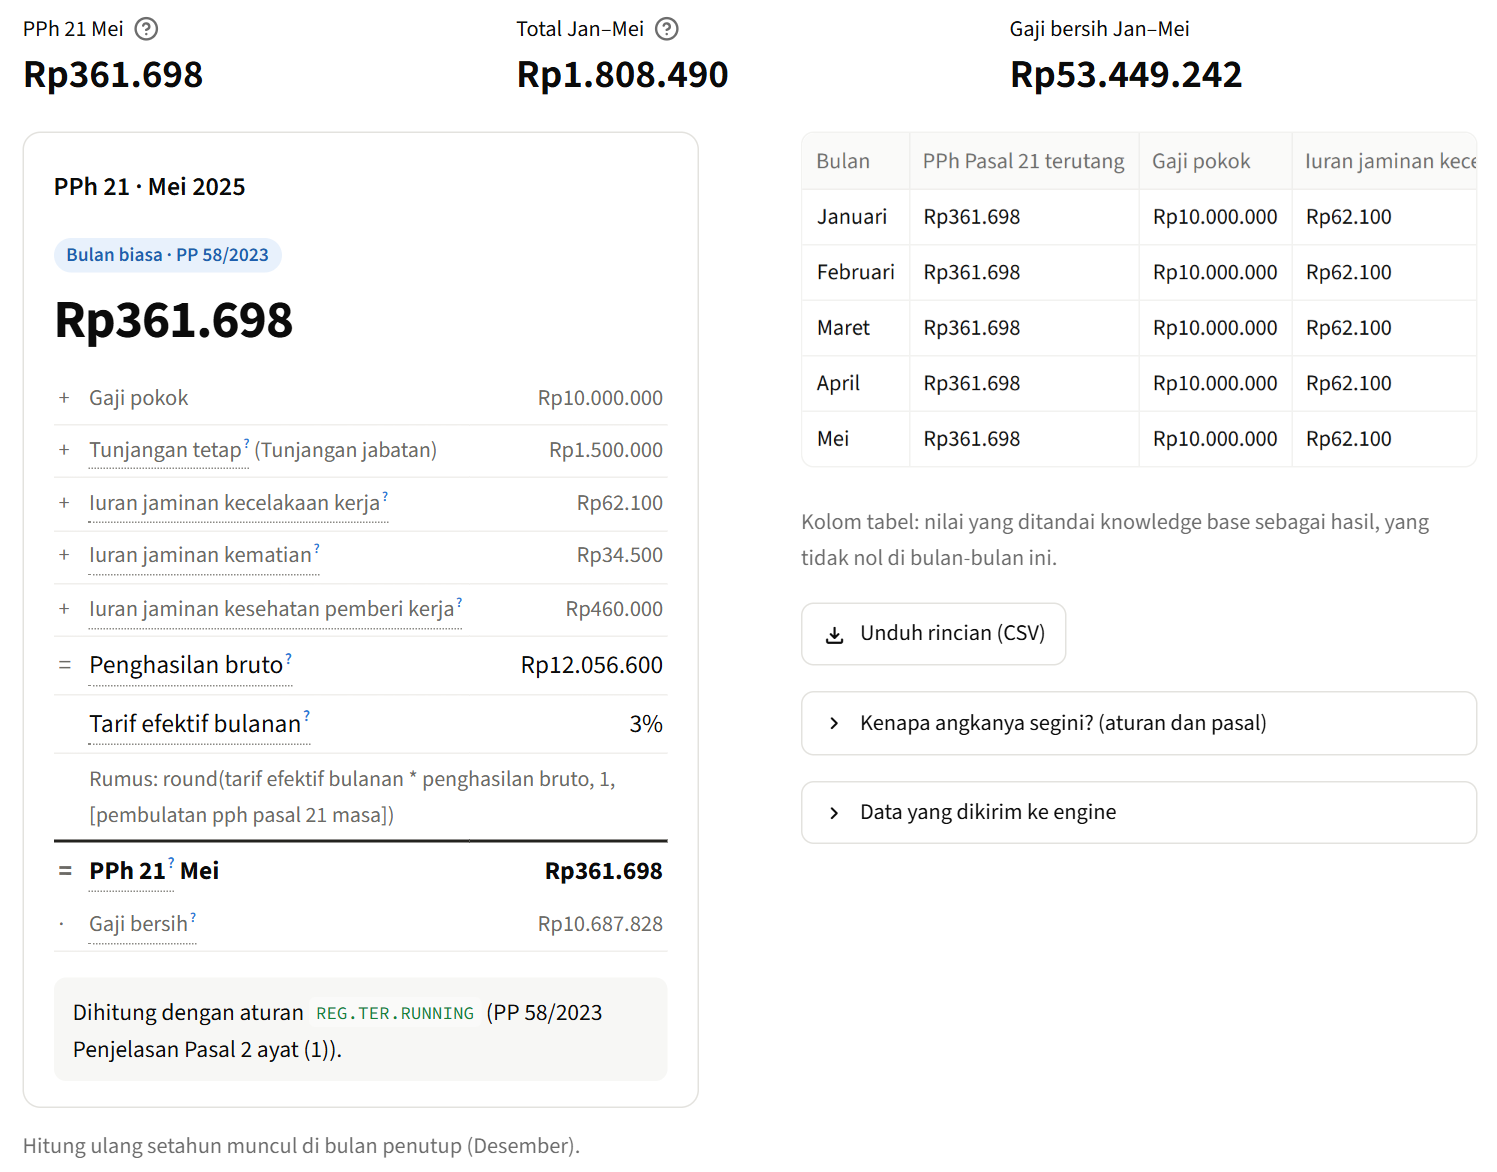
\includegraphics[width=\textwidth]{figs/screen_calculator.png}\\[1pt]{\footnotesize (a)}
\end{minipage}\hfill
\begin{minipage}[b]{0.425\textwidth}\centering
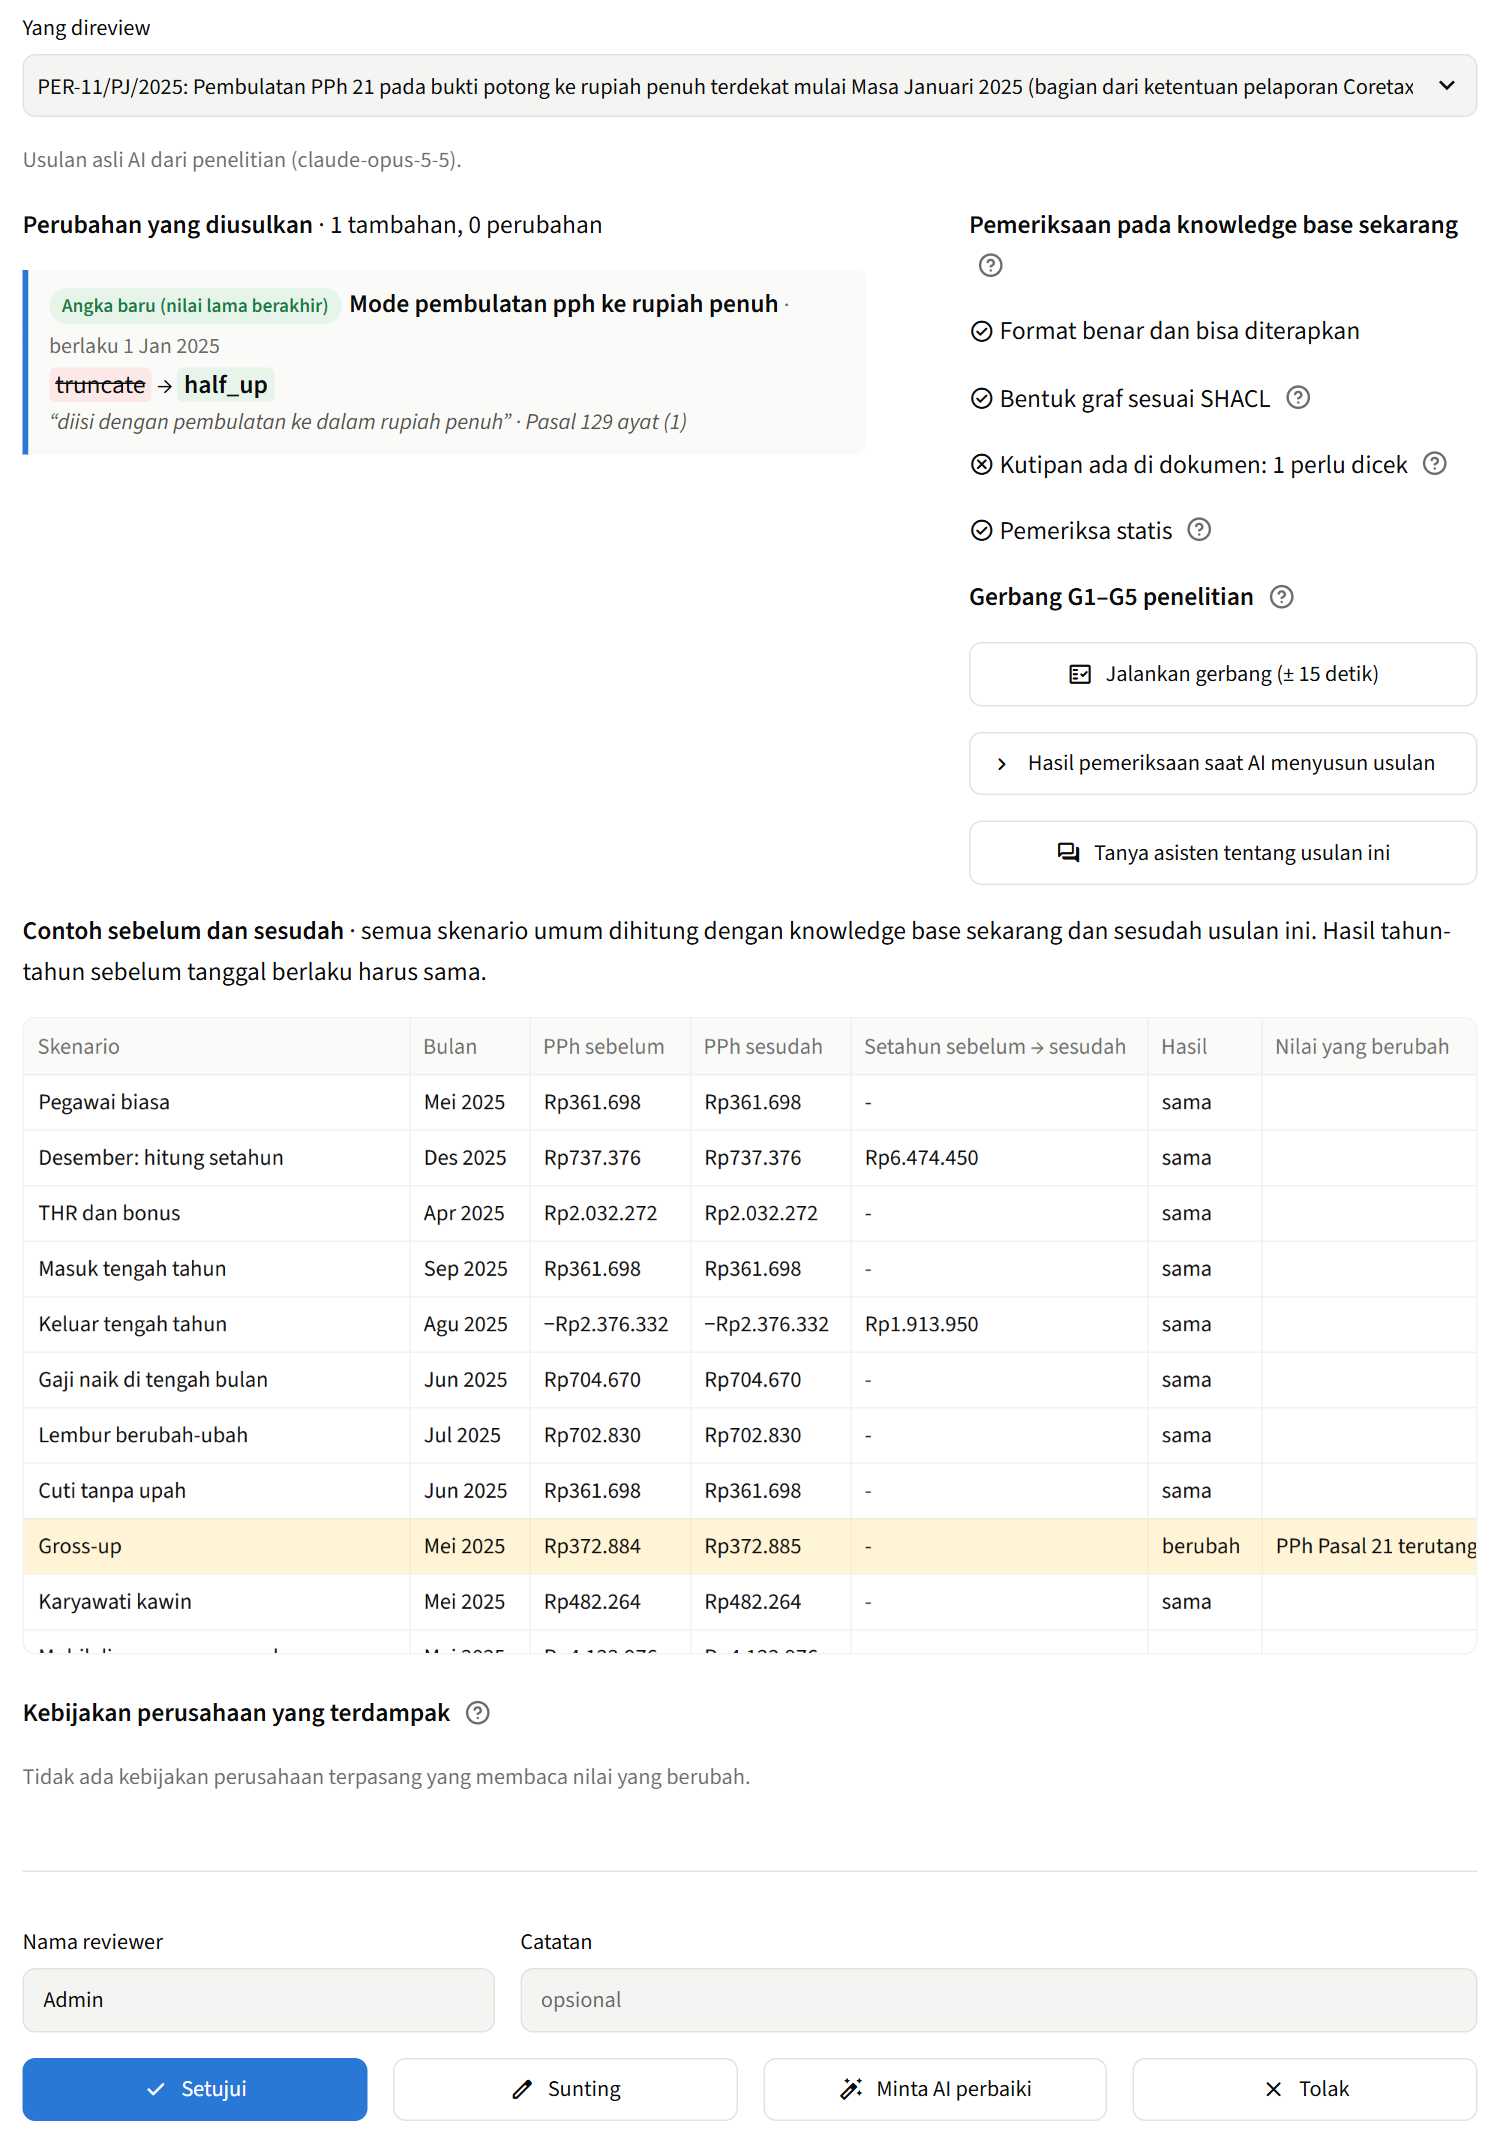
\includegraphics[width=\textwidth]{figs/screen_review.png}\\[1pt]{\footnotesize (b)}
\end{minipage}
\caption{The application, in Indonesian. (a) Calculator result for May 2025: gross income built from salary, allowance, and employer premiums, the TER rate of 3\%, PPh 21 of Rp361,698, and the rule \texttt{REG.TER.RUNNING} with its provision. (b) Review of the drafted update for PER-11/PJ/2025 (rounding mode \texttt{truncate} to \texttt{half\_up}, quoted from Article 129(1)), with the checks on the current knowledge base, before-and-after results for common scenarios (the gross-up scenario changes), affected company policies (none), and the approve, edit, repair, and reject actions.}
\label{fig:screens}
\end{figure*}
